\section{Hierarchical Clustering \label{sec:authorship_clustering_methods}}

To find clusters of authors, a possible way is to use a hierarchical clustering algorithm on a rank list.
The rank list indicate if the two documents should belong to the same cluster by order of certainty.
The hierarchical clustering regroup documents following this order.

The hardest task with this clustering scheme is to find the position in the rank list where true link become less frequent than false link.
In the clustering context, the optimal position is unknown since the true labels are not available.
We call this type of problem unsupervised.
The position should minimize the true links under it and the false links above it.

In this study, finding this position will also be referred to as finding the \textit{cut}.
We define the true positive as true links above the cut, true negatives as false links under the cut.
In addition, false positive are true links under the cut and false negatives are false links above the cut.

To find this cut, three approaches are explored: a Silhouette-based model, a distribution-based model and a regression-based model.

The Silhouette-based method can be used when only one corpus is available and no learning procedures can be applied.
This method is presented and evaluated in Section~\ref{sec:silhouette-based_clustering}.

The distribution-based model learn based on a corpus' rank list with labels (training corpus) a score where the cut should be for any new corpus' rank list (called testing corpus).
Section~\ref{sec:distribution_based_clustering} contains explanations for this method.

Finally, the regression based model, learn to estimate the rank lists links' true link probability from a corpus with labels (examples, training corpus).
The model can find the optimal cut for a new corpus' rank list (called testing corpus), by estimating the true link probabilities for each link.
This approach is explained in Section~\ref{sec:regression_based_clustering}.

\subsection{Algorithm and Implementation \label{sec:algorithm_and_implementation}}

The scikit-learn Python module \cite{sklearn} provide a bottom-up implementation of the hierarchical clustering, which is called agglomerative clustering.

The agglomerative clustering follow this procedure:
\begin{enumerate}
  \item The rank list used is converted into a 2D distances' matrix, with each link representing an element of the matrix (ref. Section~\ref{sec:distances_matrix}).
  \item At the beginning, each document is considered as a single document cluster.
  \item The link (element) with the lowest score in the matrix is used to merge the next clusters.
  \item The matrix is updated following a linkage criterion. Columns and rows of the clusters merged are updated by appling a linkage criterion.
  \item 3. and 4. can be repeated until a single cluster remain.
\end{enumerate}

Multiple linkage criteria are available:

\begin{itemize}
  \item
  \textit{Ward} : metric that aim to minimize the variance of the cluster merged
  \item
  \textit{Average-linkage} : use the average score of each link of the cluster merged
  \item
  \textit{Complete-linkage} : use the maximal score of each link of the cluster merged
  \item
  \textit{Single-linkage} : use the minimal score of each link of the cluster merged
\end{itemize}

Example~\ref{ex:agglomerative_clustering} show an example for the merging procedures and linkage criteria.

Ward linkage was discarded since the current \textit{scikit-learn} implementation only allow Euclidean distance for its computation.

The merging procedure can be stopped with one of the two following criteria:

\begin{itemize}
  \item
  When a certain cluster number is reached.
  \item
  When the lowest score for the next merge is above a certain value. This value is called the distance threshold.
\end{itemize}

The so-called cut can be associated to the distance threshold.
The cut is a theoretical position in the rank list which maximize true links above the cut and false link under.
In the other hand, the distance threshold is the score at which the algorithm should stop merging clusters.
They are not exactly the same, since when clusters are merged in the distances' matrix, the resulting distances' matrix can not be expressed as a rank list anymore.

The two supervised methods proposed in this study try to estimate the distance threshold, by estimating the optimal cut.
Once a distance threshold is estimated, the hierarchical clustering is run on the rank list and is stopped according to the distance threshold.

There is one main flaw with the current scikit-learn implementation.
It does not provide a way to access the clusters at each merging step.
This feature is required for the unsupervised method, which evaluated multiple clustering results.

A possible workaround is to run the algorithm multiple time.
Each time, the algorithm is stopped at a different number of clusters (a different step).
Though this workaround is valid, it still introduces unnecessary additional merges.
This overhead have a complexity of $O(1 + 2 + 3 + ... + n - 1) = O(\frac{n * (n - 1)}{2}) = O(n^2)$, with $n$ equal to the number of documents.
In other words, with the workaround, each time the algorithm is run, all the merges computed at the previous run must re-recomputed.
To avoid this overhead, the agglomerative clustering algorithm was reimplemented to allow access to the clusters at each step.

\begin{example}
  \caption{Agglomerative clustering}
  \label{ex:agglomerative_clustering}

  \begin{subexample}{\linewidth}
    \centering
    \subcaption{Initial clusters and their distances}
    \begin{tabular}{c|c c c c}
      \toprule
        & A & B & C & D \\
      \midrule
      A & - & \textbf{1} & $2$ & $3$ \\
      B & - & - & $8$ & $7$\\
      C & - & - & - & $6$ \\
      D & - & - & - & - \\
      \bottomrule
    \end{tabular}
  \end{subexample}

  \vspace{0.2cm}

  The link with the smallest distance is A-B with a distance of 1.
  At the next step, the clusters A and B are merged into a cluster called AB.
  (b), (c) and (d) shows how to update the distances' matrix in (a) depending on the linkage criterion.

  \vspace{0.5cm}

  \begin{subexample}{\linewidth}
    \centering
    \subcaption{First merge using single-linkage\label{ex:agglomerative_clustering_single}}
    \begin{tabular}{c|c c c}
      \toprule
        & AB & C & D \\
      \midrule
      AB & - & $\text{min} \left[2, 8 \right] = 2$ & $\text{min} \left[3, 7 \right] = 3$ \\
      C  & - & - & $6$ \\
      D  & - & - & - \\
      \bottomrule
    \end{tabular}
  \end{subexample}

  \vspace{0.2cm}

  Next step will merge AB and C.

  \vspace{0.5cm}

  \begin{subexample}{\linewidth}
    \centering
    \subcaption{First merge using average-linkage\label{ex:agglomerative_clustering_average}}
    \begin{tabular}{c|c c c}
      \toprule
        & AB & C & D \\
      \midrule
      AB & - & $\text{avg} \left[2, 8 \right] = 5$ & $\text{avg} \left[3, 7 \right] = 4$ \\
      C  & - & - & $6$ \\
      D  & - & - & - \\
      \bottomrule
    \end{tabular}
  \end{subexample}

  \vspace{0.2cm}

  Next step will merge AB and D.

  \vspace{0.5cm}

  \begin{subexample}{\linewidth}
    \centering
    \subcaption{First merge using complete-linkage\label{ex:agglomerative_clustering_complete}}
    \begin{tabular}{c|c c c}
      \toprule
        & AB & C & D \\
      \midrule
      AB & - & $\text{max} \left[2, 8 \right] = 8$ & $\text{max} \left[3, 7 \right] = 7$ \\
      C  & - & - & 6 \\
      D  & - & - & - \\
      \bottomrule
    \end{tabular}
  \end{subexample}

  \vspace{0.2cm}

  Next step will merge C and D.
\end{example}


\subsection{Parameters\label{sec:hierarchical_clustering}}

As explained in Section~\ref{sec:algorithm_and_implementation}, the hierarchical clustering decide clusters based on a bottom-up approach and have two main parameters, the stopping procedure and the linkage criterion.
The linkage criterion can be: single, average or complete linkage.
Oxquarry, Brunet, St-Jean A, St-Jean B and St-Jean corpora are used for this experiment.

The goal is to understand how the linkage criterion behave for the best clustering achievable (best $B^3_{F_1}$).

The custom implementation of the hierarchical clustering is used, at each merging step, the intermediary clustering is evaluated using the $B^3_{F_1}$.
The clustering resulting in the best $B^3_{F_1}$ is kept.
For each linkage criteria, corpus and text representation clustering and its evaluation is achieved.

The results are presented in Table~\ref{tab:hierarchical_clustering}.

These results can be considered as the $B^3_{F_1}$ upper bound for the hierarchical clustering using these rank lists on these corpora.
We refer to them as \textit{upper bound} or \textit{rank lists upper bound}.

The best linkage criterion depends on the corpus, but in average, the best $B^3_{F_1}$ is achieved with the average linkage criterion.
The average linkage is $\sim 1\%$ better than the complete linkage and $\sim 6\%$ better than the single linkage.

We assumed that the better the rank list are, the better the clustering result is when applying the hierarchical clustering.
This assumption can be verified in Figure~\ref{fig:correlation_average_precision_b3f1}.
In this Figure, we compare the average precision (AP) of each retained rank list to the $B^3_{F_1}$ of the best clustering obtainable with the hierarchical clustering on this rank list (ref. Table~\ref{tab:hierarchical_clustering}).

We can clearly observe a linear relationship between the average precision and the $B^3_{F_1}$.
The linear regression for the single linkage have an r-value of $10^{-11}$, $10^{-12}$ for the average linkage and $10^{-6}$ for the complete linkage.
This result further motivate this assumption.

\begin{figure*}
  \centering
  \caption{Evaluation methodology for the clustering}
  \label{fig:clustering_evaluation_methodology}
  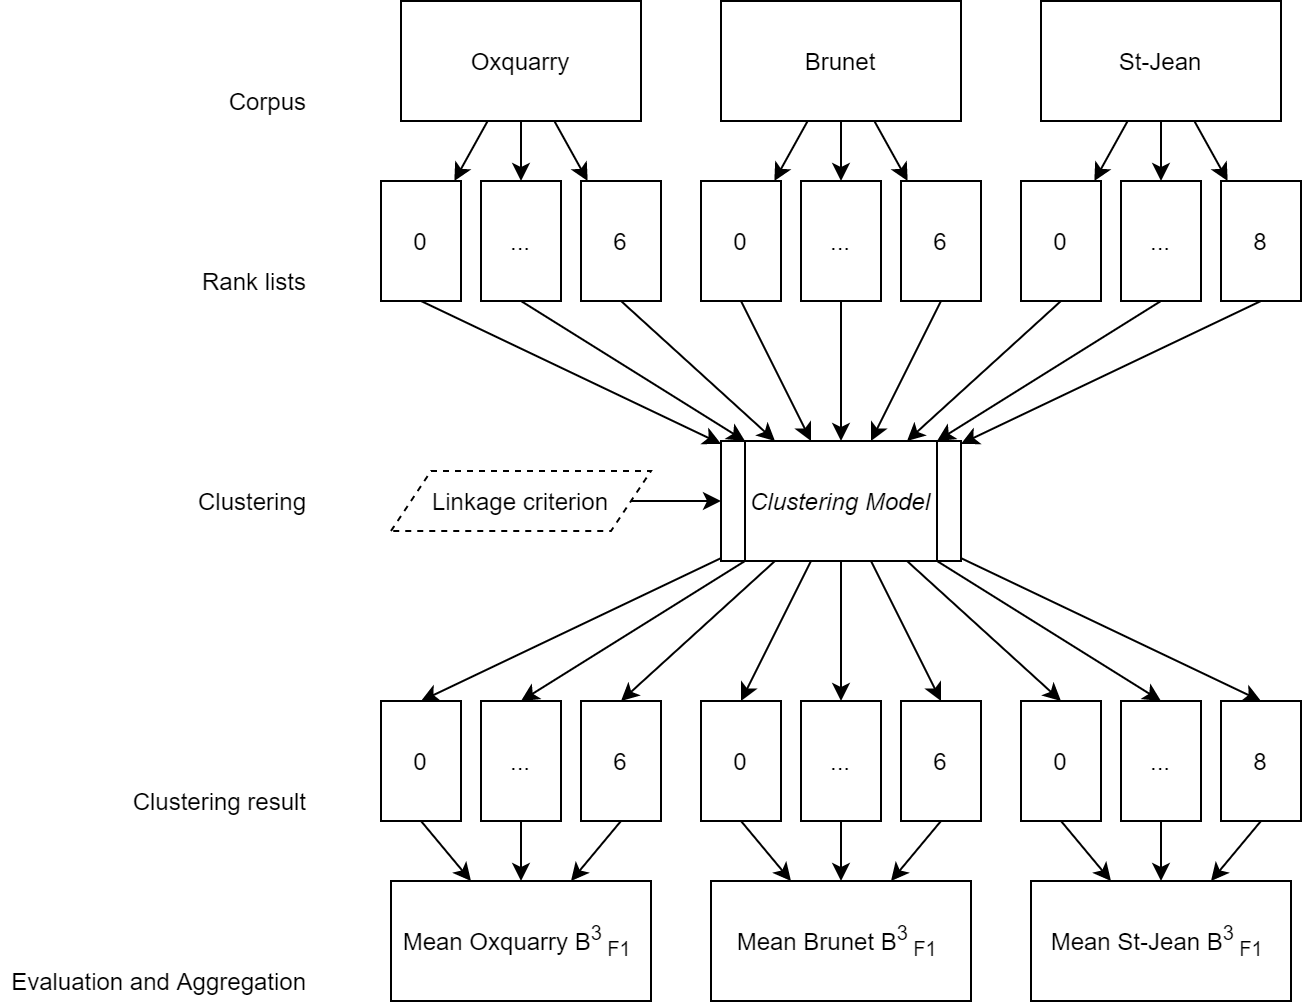
\includegraphics[width=0.7\linewidth]{img/clustering_evaluation_methodology.png}
\end{figure*}

\begin{table}
  \centering
  \caption{Best $B^3_{F_1}$ with hierarchical clustering on every rank lists and linkage criterion}
  \label{tab:hierarchical_clustering}

  \resizebox{\linewidth}{!}{
  \begin{tabular}{l l c c c}
    \toprule
    \multicolumn{2}{c}{Rank list} & \multicolumn{3}{c}{Linkage criterion} \\
    TR ID & Corpus & Single & Average & Complete \\
    \midrule
    0 & Oxquarry & 0.95 & 1.00 & 0.90 \\
    1 & Oxquarry & 0.93 & 0.93 & 0.82 \\
    2 & Oxquarry & 0.67 & 0.74 & 0.80 \\
    3 & Oxquarry & 0.77 & 0.77 & 0.84 \\
    4 & Oxquarry & 0.87 & 0.91 & 0.84 \\
    5 & Oxquarry & 0.88 & 0.89 & 0.84 \\
    6 & Oxquarry & 0.86 & 0.83 & 0.80 \\
    \midrule
    \multicolumn{2}{l}{Oxquarry mean} & 0.85 & 0.87 & 0.84 \\
    \midrule
    0 & Brunet & 0.81 & 0.82 & 0.77 \\
    1 & Brunet & 0.82 & 0.85 & 0.89 \\
    2 & Brunet & 0.77 & 0.84 & 0.77 \\
    3 & Brunet & 0.79 & 0.80 & 0.78 \\
    4 & Brunet & 0.78 & 0.82 & 0.81 \\
    5 & Brunet & 0.79 & 0.82 & 0.90 \\
    6 & Brunet & 0.86 & 0.82 & 0.87 \\
    \midrule
    \multicolumn{2}{l}{Brunet mean} & 0.80 & 0.83 & 0.83 \\
    \midrule
    0 & St-Jean A & 0.82 & 0.89 & 0.91 \\
    1 & St-Jean A & 0.77 & 0.84 & 0.88 \\
    2 & St-Jean A & 0.78 & 0.87 & 0.91 \\
    3 & St-Jean A & 0.80 & 0.82 & 0.83 \\
    4 & St-Jean A & 0.68 & 0.86 & 0.89 \\
    5 & St-Jean A & 0.74 & 0.88 & 0.91 \\
    6 & St-Jean A & 0.76 & 0.88 & 0.87 \\
    7 & St-Jean A & 0.69 & 0.83 & 0.77 \\
    8 & St-Jean A & 0.81 & 0.84 & 0.82 \\
    \midrule
    \multicolumn{2}{l}{St-Jean A mean} & 0.76 & 0.86 & 0.86 \\
    \midrule
    0 & St-Jean B & 0.93 & 0.95 & 0.95 \\
    1 & St-Jean B & 0.91 & 0.94 & 0.96 \\
    2 & St-Jean B & 0.94 & 0.98 & 0.96 \\
    3 & St-Jean B & 0.94 & 0.95 & 0.91 \\
    4 & St-Jean B & 0.93 & 0.95 & 0.91 \\
    5 & St-Jean B & 0.94 & 0.95 & 0.94 \\
    6 & St-Jean B & 0.87 & 0.90 & 0.93 \\
    7 & St-Jean B & 0.91 & 0.95 & 0.90 \\
    8 & St-Jean B & 0.91 & 0.95 & 0.93 \\
    \midrule
    \multicolumn{2}{l}{St-Jean B mean} & 0.92 & 0.95 & 0.93 \\
    \midrule
    \multicolumn{2}{l}{Absolute mean} & 0.83 & 0.88 & 0.87 \\
    \bottomrule
  \end{tabular}
  }

  \vspace{0.2cm}

  \textit{TR: Text representation}
\end{table}

\begin{figure}
  \caption{Optimal clustering $B^3_{F_1}$ correlation with rank list AP}
  \label{fig:correlation_average_precision_b3f1}

  \subcaption{Single Linkage}
  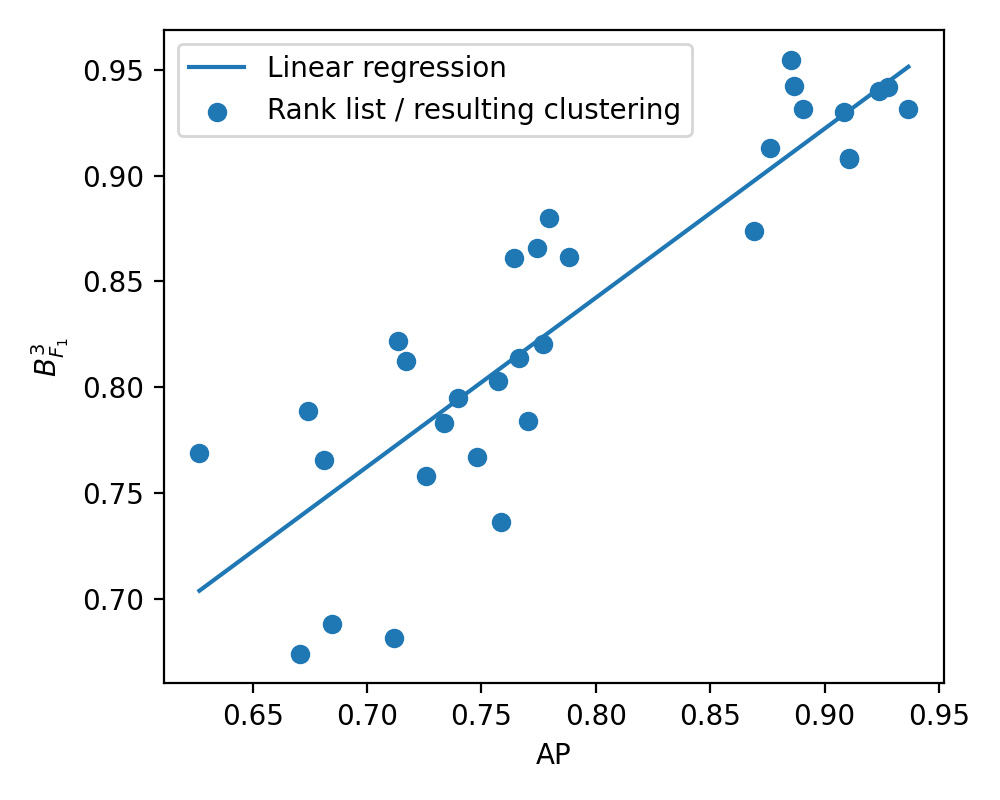
\includegraphics[width=\linewidth]{img/correlation_average_precision_b3f1_0.png}
  \subcaption{Average Linkage}
  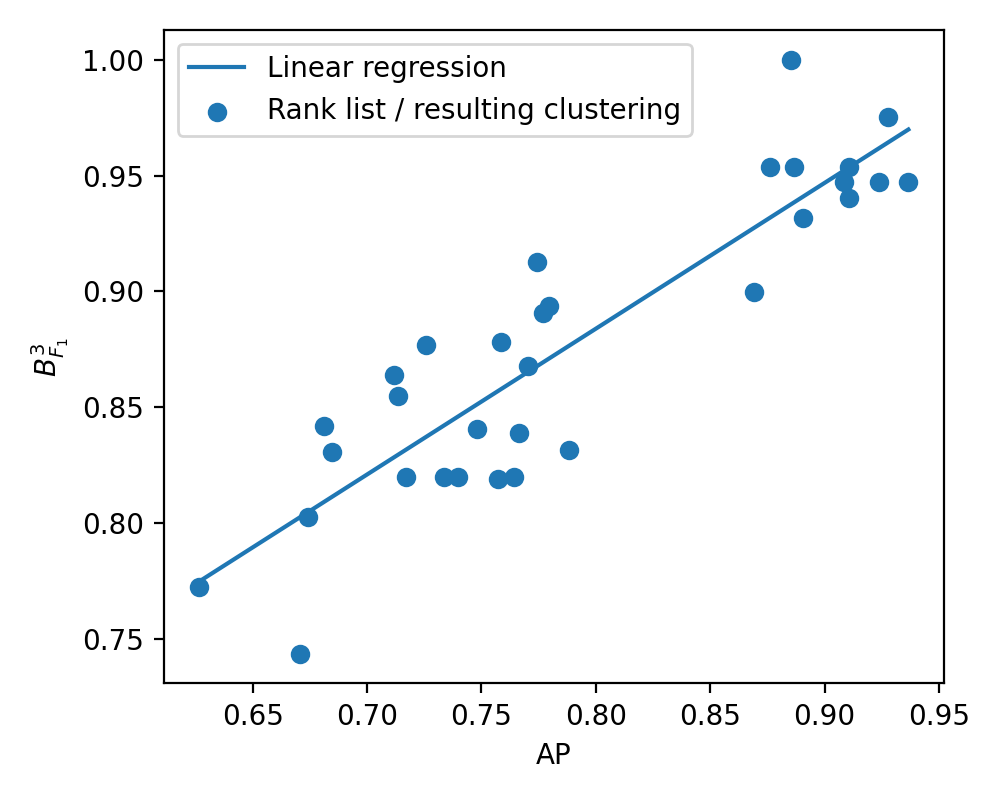
\includegraphics[width=\linewidth]{img/correlation_average_precision_b3f1_1.png}
  \subcaption{Complete Linkage}
  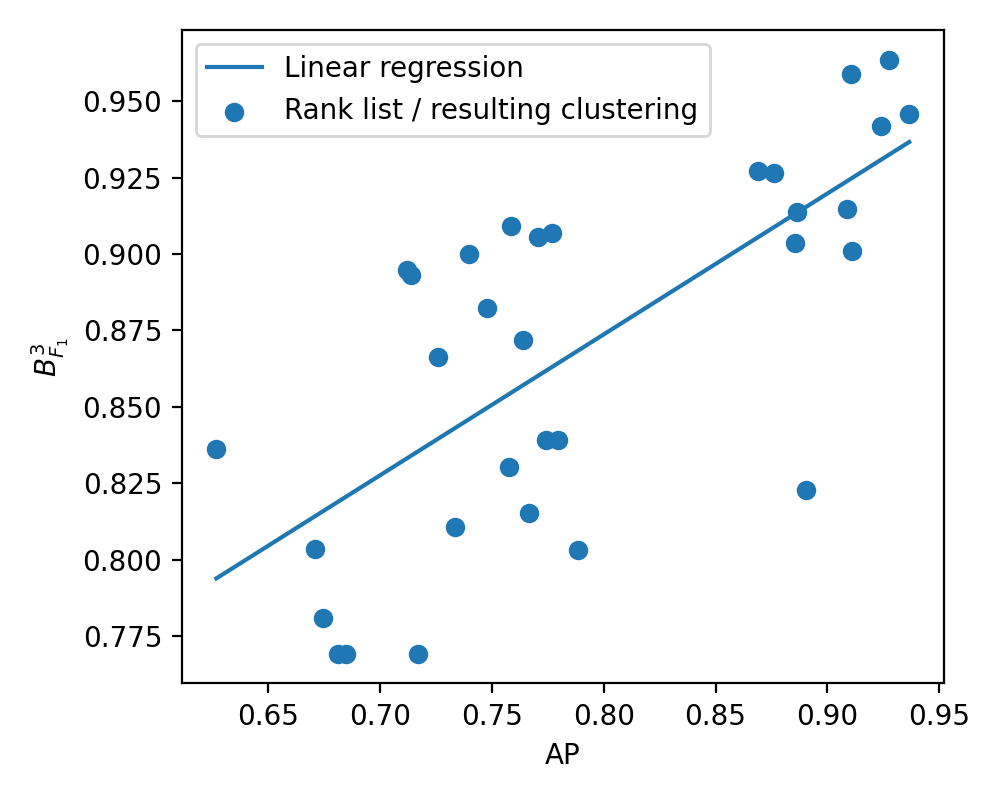
\includegraphics[width=\linewidth]{img/correlation_average_precision_b3f1_2.png}
\end{figure}
